\documentclass[12pt]{article}
\usepackage[table]{xcolor}
\usepackage[shortlabels]{enumitem}
\usepackage{tabularx,xltabular}
\usepackage{graphicx}
\usepackage{hyperref}
\usepackage{verbatim}
\usepackage{geometry}
\usepackage{ulem}
\usepackage[official]{eurosym}
\usepackage{tikz}
\usetikzlibrary{arrows,backgrounds,calc,decorations.markings,patterns,3d}
\usepackage{pgfplots}
\pgfplotsset{compat = newest}
\usetikzlibrary{fit}
\newcommand\addvmargin[1]{
\usetikzlibrary{arrows}
\node[fit=(current bounding box),inner ysep=#1,inner xsep=0]{};}
\usepackage{cancel}
\usepackage{fontspec}
\usepackage{array}  
\geometry{a4paper, top=2cm, left=2cm, right=2cm, bottom=2cm, headsep=1cm}
\usepackage{tabu}
\usepackage{pst-node}
\usepackage{colortbl}
\usepackage{array}
\usepackage{german}
\setlength\parindent{0pt}
\newcolumntype{?}{!{\vrule width 1pt}}
\usepackage{makecell}
\usepackage{pbox}
\usepackage{amssymb}
\usepackage{amsmath}
\usepackage{booktabs}
\newcolumntype{L}[1]{>{\raggedright\let\newline\\\arraybackslash\hspace{0pt}}m{#1}}
\newcolumntype{C}[1]{>{\centering\let\newline\\\arraybackslash\hspace{0pt}}m{#1}}
\newcolumntype{R}[1]{>{\raggedleft\let\newline\\\arraybackslash\hspace{0pt}}m{#1}}
\begin{document}
\rightline{}
\centerline{{\Large }} 
\vspace{1cm}
\noindent \\


\tikzstyle{background grid}=[draw, black!15,step=.5cm]
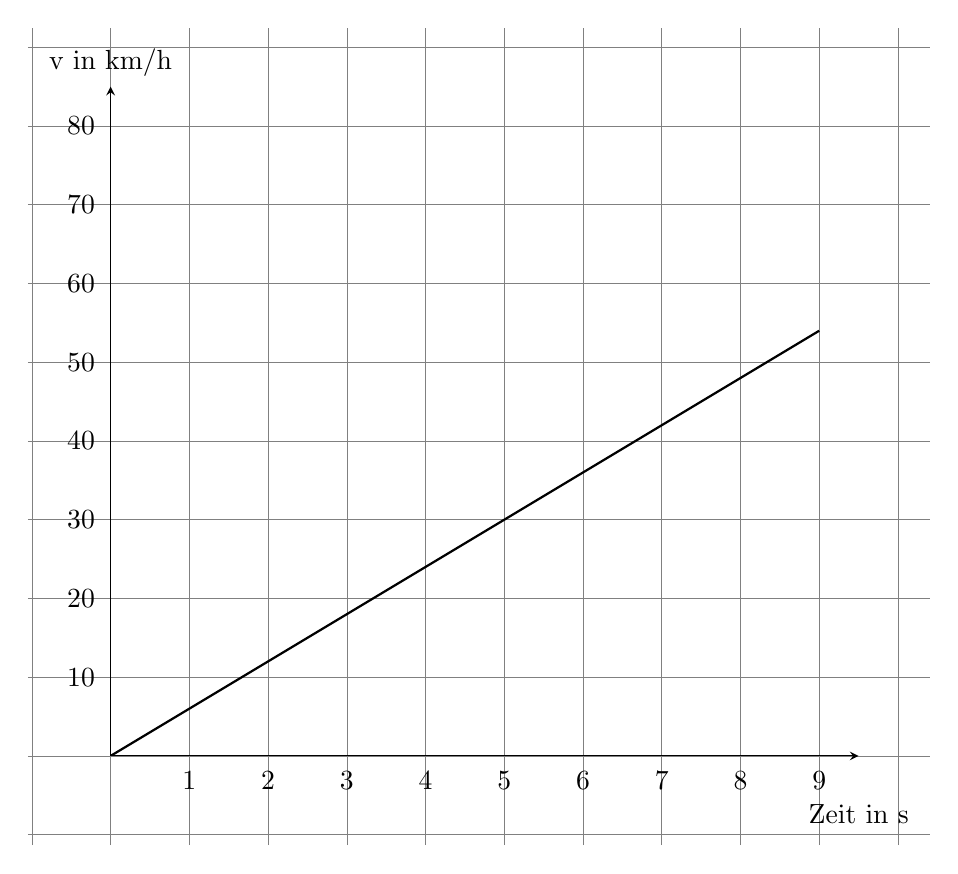
\begin{tikzpicture}[show background grid]
\begin{axis}[    axis lines = middle, scale only axis=true, at={(0cm,0cm)},
    width=9.5 cm, xmin = 0.0, xmax = 9.5,xtick distance = 1.0,
    height=8.5cm, ymin = 0.0, ymax = 85.0, ytick distance = 10.0,
    xlabel = {Zeit in s},x label style={at={(current axis.right of origin)},anchor=north, below=5mm},
    ylabel = {v in km/h},y label style={at={(current axis.above origin)},anchor=south}]
    \addplot[domain = 0:9,samples = 200,smooth,thick,black ] { (6*x)};
\end{axis}
\end{tikzpicture}
\\
\tikzstyle{background grid}=[draw, black!15,step=.5cm]
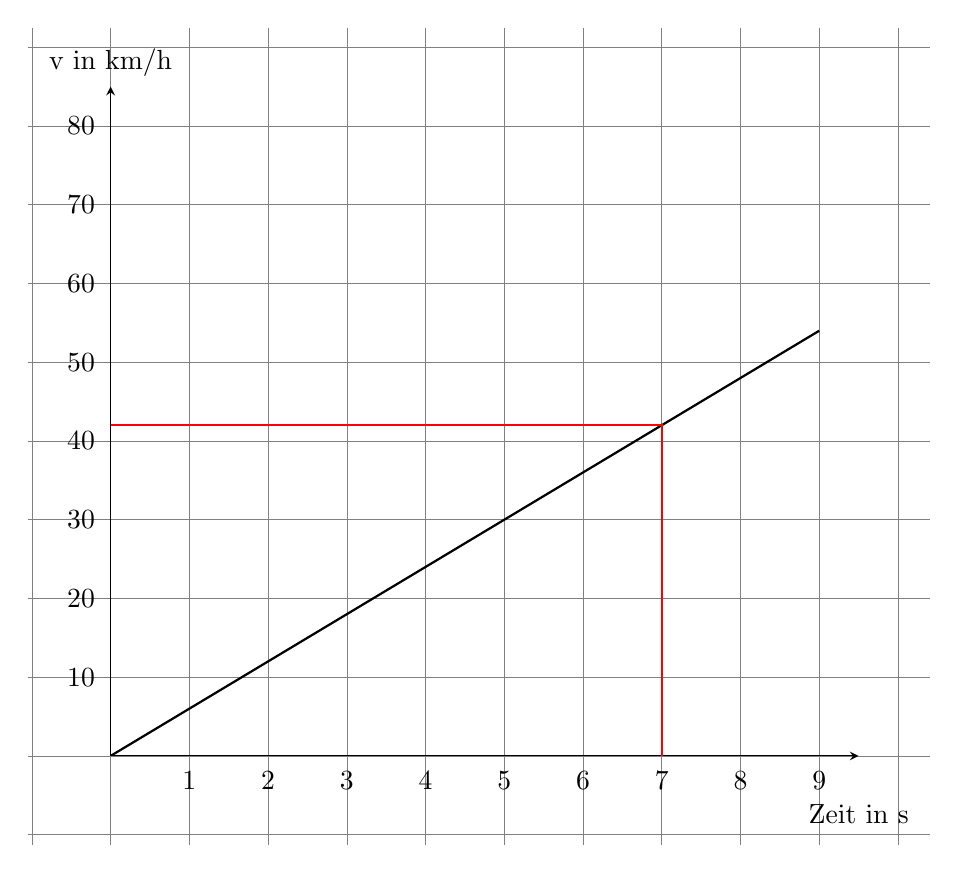
\begin{tikzpicture}[show background grid]
\begin{axis}[    axis lines = middle, scale only axis=true, at={(0cm,0cm)},
    width=9.5 cm, xmin = 0.0, xmax = 9.5,xtick distance = 1.0,
    height=8.5cm, ymin = 0.0, ymax = 85.0, ytick distance = 10.0,
    xlabel = {Zeit in s},x label style={at={(current axis.right of origin)},anchor=north, below=5mm},
    ylabel = {v in km/h},y label style={at={(current axis.above origin)},anchor=south}]
    \addplot[domain = 0:9,samples = 200,smooth,thick,black ] { (6*x)};
    \addplot[thick, color=red] coordinates {  (7,0) (7,42) (0,42) };
\end{axis}
\end{tikzpicture}
\end{document}